\chapter{Idler-frame case study}\label{chap:chapter3}

In this chapter, I apply the methods and learnings from chapter~\ref{chap:chapter2} to an industry dataset of the failure times of idler-frames on an overland iron ore conveyor. The idler-frames were described briefly in sections~\ref{sec:industry-data}. For a reliability engineer tasked with maintaining the conveyor, it can be useful to quantify the expected failure times of the idler-frames currently in operation and the expected number of failures in the next short time interval, such as \citet{hong2009} do for power transformers. I show how these quantities are already naturally contained in the full posterior of the Bayesian model when the censored lifetimes are imputed as in sec.~\ref{subsec:censoring-treatments}. It is also useful to propagate uncertainty in the posterior estimates of the parameters through any decision criteria to understand risk in long-term maintenance plans, such as the design of a fixed-time replacement strategy. I demonstrate how the joint posterior draws of the Weibull parameters can be propagated through a cost function to make an informed decision about a fixed-time replacement strategy for the idlers in the frames.

The chapter is structured as follows. Section~\ref{sec:idler-frame-data-desc} describes the data in detail. In Section~\ref{sec:idler-frame-joint-prior}, I construct an informative prior for the idler-frame analysis based on prior knowledge supplied by the idler manufacturer and a conveyor engineer. Section~\ref{sec:idler-frame-posterior} describes the model fitting process and posterior inference on the parameters. Section~\ref{sec:idler-frames-using-posterior} goes on to demonstrate how the draws from the posterior can be used. Specifically, subsections~\ref{subsec:idler-FTs} and~\ref{subsec:idler-cumulative-failrues} show how to obtain the estimated remaining useful life of the currently installed idler-frames and the expected number of failures in a time interval following the end of observation, respectively. Subsection~\ref{subsec:idler-cost-function} then shows how to propagate the posterior uncertainty about the lifetime distribution through utility functions---specifically a cost function---to inform the choice of a preventative replacement interval for the idler-frames. Finally, section~\ref{sec:idler-frame-conclusions} summarises and concludes the chapter.

\section{Idler-frame lifetime data} \label{sec:idler-frame-data-desc}

The data is a synthesis of preventative and reactive replacement records of idlers on a single overland iron ore conveyor. It is one of many such datasets for similar conveyors on the mine. This specific conveyor has one hundred and forty-three frames of idlers, each with a three-idler configuration. When an idler in the frame fails, all three of the idlers are typically replaced, so each idler frame can be viewed as one unit. The replacements of the idlers in a frame are typically captured in the CMMS, and if an idler in the frame has been observed as failed and scheduled to be replaced, then this information is included in the replacement record. However, if an idler in the frame has failed in a way that threatens to damage the belt immediately, then this is raised in a different system, the belt is shut down, and the idlers in that frame are replaced. During an industry placement, I cleaned and collated these different sources of replacement records into a single dataset. The dataset spans just over six years, but the conveyor has been in operation for twenty.

From the replacement records, the lifetimes of the idler-frames can be calculated as the time between the replacements. However, since the records do not go back to the commissioning of the conveyor, the first observed lifetime for each frame is left truncated and has unknown installation time. Because the sets of idlers in some frames are preventatively replaced or because some were still in operation when I constructed the dataset, there are many right censored lifetimes. Table~\ref{tab:idler-frame-summary} gives an overview of the dataset of idler frame lifetimes, and Figure~\ref{fig:idler-frames-data} shows the lifetimes of each frame along the conveyor. In Fig.~\ref{fig:idler-frames-data}, the fully observed lifetimes---i.e. we observed the failure of an idler in the frame as well as the previous failure for that frame---are shown as orange points, while the partially observed lifetimes are shown in blue. The partially observed lifetimes that are left-truncated by the beginning of the observation period are shown as triangular points, while the remainder of the blue points are right-censored observations.

\begin{table}
\centering
\caption{\label{tab:idler-frame-summary}Summary of the idler frame data set.}
\centering
\begin{tabular}[t]{ll}
\toprule
\cellcolor{gray!10}{Maximum lifetime} & \cellcolor{gray!10}{2167 days}\\
Minimum lifetime & 1 days\\
\cellcolor{gray!10}{Maximum fully observed lifetime} & \cellcolor{gray!10}{1461 days}\\
Beginning of observation & 2014-12-10\\
\cellcolor{gray!10}{End of observation} & \cellcolor{gray!10}{2020-11-15}\\
\addlinespace
Number of observations & 402\\
\cellcolor{gray!10}{Number of unique frames} & \cellcolor{gray!10}{143}\\
Number of left truncated observations & 143\\
\cellcolor{gray!10}{Number of right censored observations} & \cellcolor{gray!10}{144}\\
Number of left truncated and right censored observations & 1\\
\bottomrule
\end{tabular}
\end{table}


Table~\ref{tab:idler-frame-summary} shows that roughly thirty-six per cent of the lifetimes in the dataset are left-truncated with unknown installation times. Therefore, if we were to discard these observations, we would throw away a third of the data. Hence, we should retain the information in these left-truncated lifetimes.

Based on our understanding of how the idler-frames fail and from the characteristics of the dataset described in table~\ref{tab:idler-frame-summary}, it is appropriate to use the methods that I developed in Chap.~\ref{chap:chapter2} to analyse the industry dataset and impute the partially observed truncated lifetimes. The Weibull distribution appears appropriate to model the idler-frame lifetimes since the idlers in the frame should fail via a wear-out failure mechanism. Furthermore, the frame's failure time is when the first idler in the frame fails, which aligns with the extreme value distribution characteristic of the Weibull (which I discussed in section~\ref{subsec:weibull-dist}). The observation period spans just over six years, and it starts roughly 14 years after the conveyor is commissioned. According to domain knowledge, the expected lifetime of an idler is roughly five years, and since the lifetime of a frame is the first of the three idlers to fail, the expected lifetime of a frame should be a little under this value. Hence, the observation window is greater than the expected lifetime, and the time from the commissioning of the conveyor to the start of the observation period is roughly three times greater. Furthermore, only one lifetime is left-truncated/interval-censored by the beginning of the observation window and right-censored by its end. Under these circumstances, it is acceptable to use the methods proposed in Chap~\ref{chap:chapter2} to account for the lifetimes that are left-truncated with unknown exposure history.

In the industry dataset, there are some very short lifetimes---twenty-five that are less than three weeks---that most likely arise from manufacturing defects or incorrect installation. In this analysis, I want to model the wear-out failure mechanism of the idler frames, and therefore, I treat any lifetimes shorter than three weeks as right censoring events; this is done by \citet{hong2009} in their analysis of power transformers---i.e. the failure due to wear was right censored by the early failure from another cause.

\begin{figure}
  \centering
  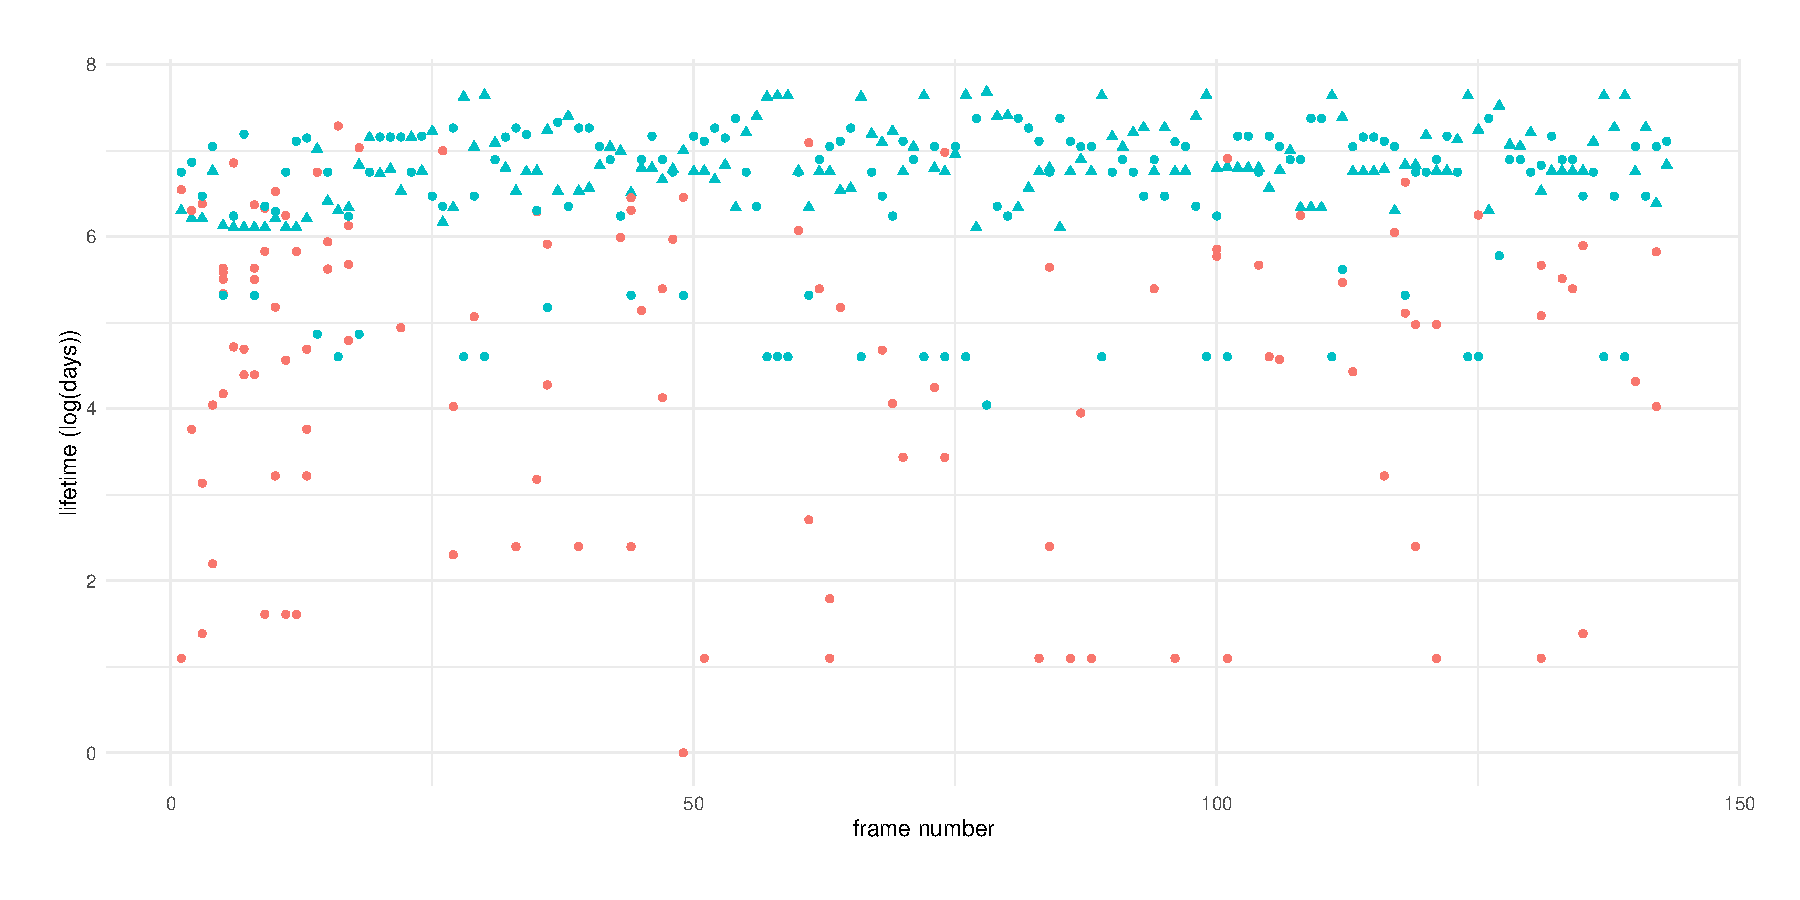
\includegraphics[width=1\textwidth]{./figures/ch-3/idler-frame-data.pdf}
  \caption{The idler-frame lifetimes plotted along the length of the conveyor. On the horizontal axis is the frame number that the lifetimes belong to, and on the vertical is the log value of the lifetime in log-days. The fully observed lifetimes are red points, while the partially observed (censored) lifetimes are blue. The censored lifetimes that are left-truncated by the start of the observation period are shown as triangular points.}
  \label{fig:idler-frames-data}
\end{figure}

\section{An informative prior} \label{sec:idler-frame-joint-prior}

Based on engineering knowledge and information provided by the manufacturer, I construct an informative joint prior for the idler-frames to supplement the analysis. According to the manufacturer, the expected lifetime of an idler is five years, and according to conveyor engineers, it is unlikely that they will last longer than eight. I express this information as the expectation of the CDF at $t_1 = 5 \times 365 = 1825$ and $t_2 = 8 \times 365 = 2920$ encoded as normal distributions, as in sec.~\ref{sec:weibull-joint-prior}. The expected value of the CDF at $t_1 = 1825$ is $0.50$, and the standard deviation is $0.15$, while the expected value of the CDF at $t_2 = 2920$ is $0.95$ with a standard deviation of $0.05$. I set the standard deviations relatively large since the expected lifetime of a frame of idlers is actually the expected smallest value of the three idlers in the frame. The resulting informative joint prior is shown if figure~\ref{fig:idler-frames-prior}, plot~(a) shows three thousand joint draws of the shape $\beta$ and scale $\eta$ from the informative prior, and plot~(b) shows the resulting prior uncertainty in the CDF.

\begin{figure}
  \centering
  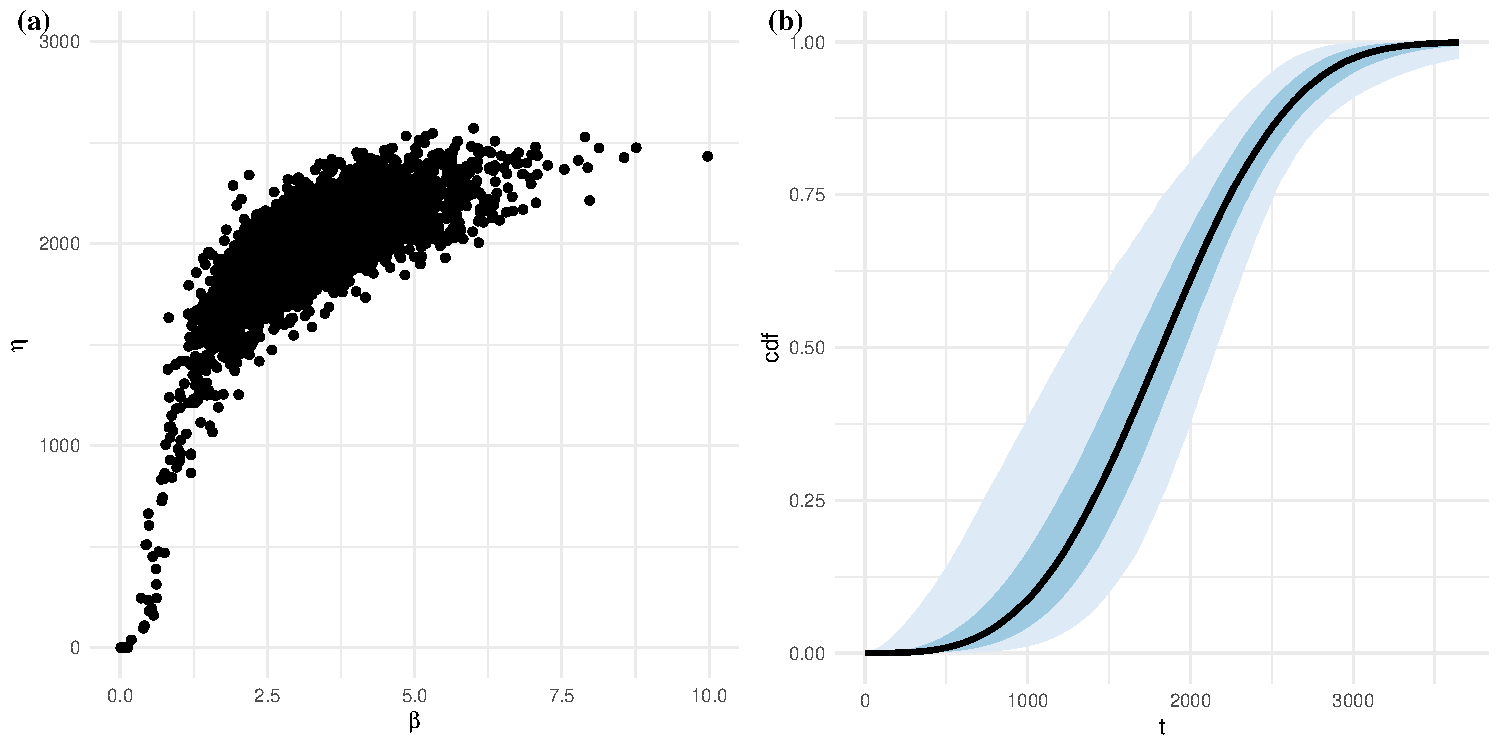
\includegraphics[width=1\textwidth]{./figures/ch-3/idler-frame-prior.pdf}
  \caption{The joint informative prior from eliciting information at $t_1 = 1825$ and $t_2 = 2920$. (a) shows 3000 draws from the informative joint prior, and (b) shows the resulting uncertainty surrounding the CDF.}
  \label{fig:idler-frames-prior}
\end{figure}

\section{Posterior draws} \label{sec:idler-frame-posterior}

To perform inference, I draw $6000$ samples from the posterior using four chains, each $2000$ iterations long and with a burn-in of $500$ iterations and no thinning using Stan \citep{Stan2022}. The Stan output summarising the joint posterior draws of $\beta$ and $\eta$ is shown in Table~\ref{tab:idler-frame-posterior-summary} and the joint draws are plotted in Figure~\ref{fig:idler-frames-post}~(a). Sampling is efficient with no divergences, the chains mix well---indicated by $\hat{R}$ values of $\approx 1$---and both parameters have a large number of effective samples. The posterior mean of the shape is just above one ($1.10$), but there is a small amount of mass just below one, and the posterior mean of the scale is $1363$. These values of the parameters yield an average frame lifetime of $1315$ days ($3.6$ years), which is significantly smaller than the recommended average lifetime of an idler provided by the manufacturer---which was five years.

\begin{table}
\centering
\caption{\label{tab:idler-frame-posterior-summary}Summary of sampling for $\beta$ and $\eta$.}
\centering
\begin{tabular}[t]{lrrrrrr}
\toprule
Parameter & Mean & 2.5\% & 50\% & 97.5\% & $n_{\small{\mbox{eff}}}$ & $\hat{R}$\\
\midrule
\cellcolor{gray!10}{$\beta$} & \cellcolor{gray!10}{1.10} & \cellcolor{gray!10}{1.01} & \cellcolor{gray!10}{1.10} & \cellcolor{gray!10}{1.20} & \cellcolor{gray!10}{5337} & \cellcolor{gray!10}{1.0001}\\
$\eta$ & 1362.56 & 1200.58 & 1361.17 & 1535.58 & 4386 & 1.0003\\
\bottomrule
\end{tabular}
\end{table}


\begin{figure}
  \centering
  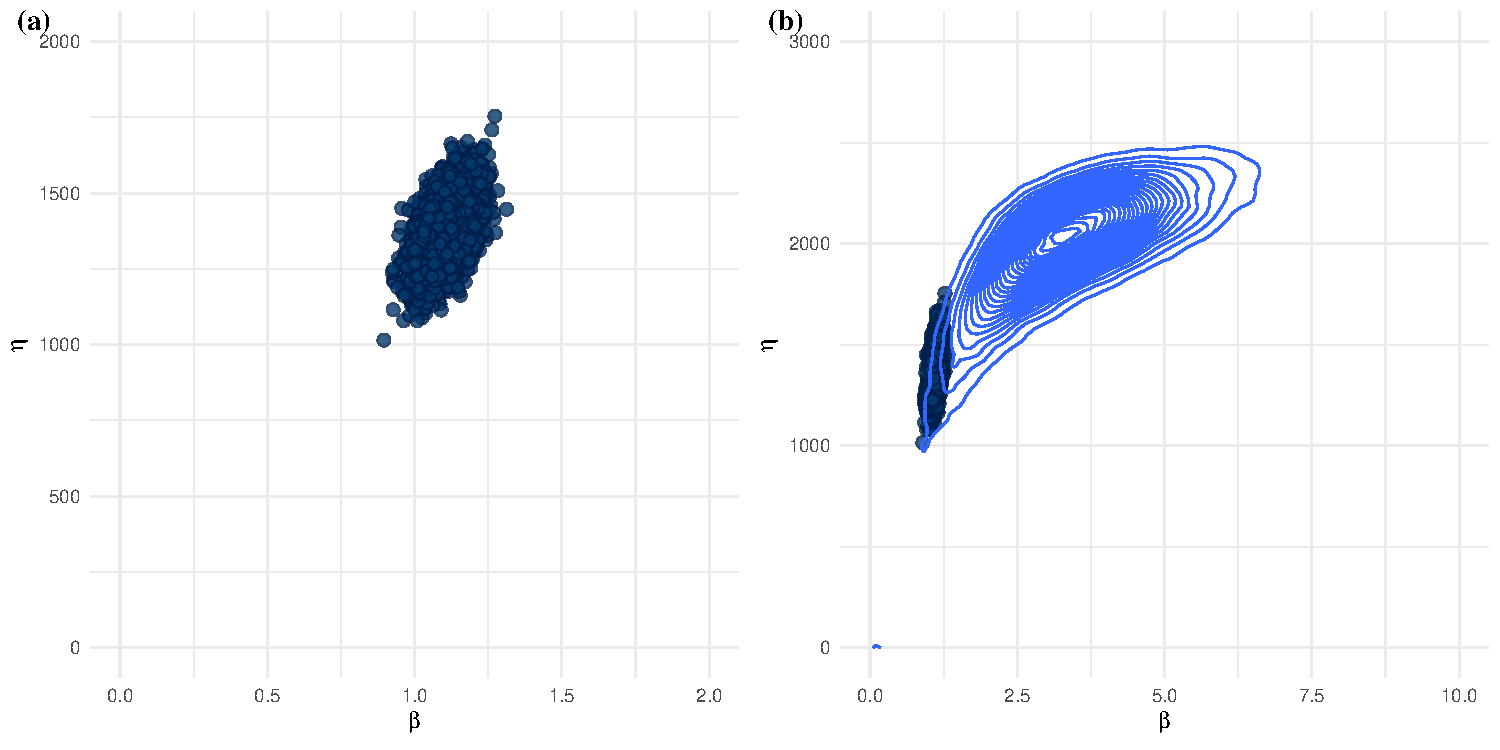
\includegraphics[width=1\textwidth]{./figures/ch-3/idler-frame-post.pdf}
  \caption{The joint draws of the Weibull parameters $\beta$ and $\eta$ from the posterior distribution. (a) shows the plain draws, and (b) compares the draws with the contours of the informative joint prior.}
  \label{fig:idler-frames-post}
\end{figure}

Figure~\ref{fig:idler-frames-post}~(b) compares the draws from the posterior with the informative joint prior. The posterior draws sit far in the tail of the joint prior but are still contained in the prior. The likelihood is strong enough that the inference about the shape and scale are fairly invariant to changes in the prior, although I do not show this here. Figure~\ref{fig:idler-frames-post-cdf} shows the refined uncertainty around the CDF that results from the posterior. The uncertainty surrounding the CDF of the lifetime distribution in the figures is much more refined compared with the prior. The estimates of the CDF at our elicitation times---$t_1 = 1825$ days and $t_2 = 2920$ days---are now $0.75$ and $0.90$, respectively. These new estimates sit in the tails of the distributions I specified to construct the prior. The discrepancy between the prior and the posterior indicates a slight prior-likelihood conflict; however, the likelihood is strong enough, in this case, to not be too influenced by the prior, and the prior does appear to have some mass around the final model.
\marginnote{\small{\textcolor{red}{Link this to next section.}}}
\begin{figure}
  \centering
  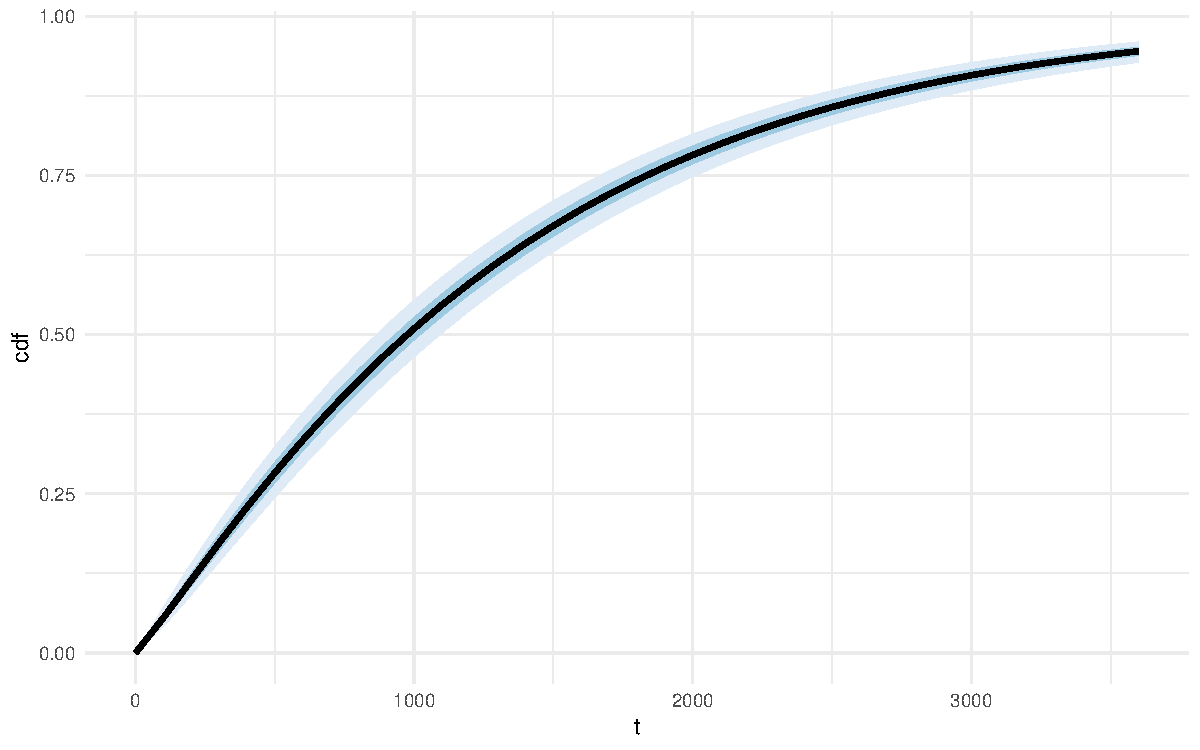
\includegraphics[width=0.7\textwidth]{./figures/ch-3/idler-frame-post-CDF.pdf}
  \caption{The resulting posterior uncertainty surrounding the Weibull CDF.}
  \label{fig:idler-frames-post-cdf}
\end{figure}

\section{Using the posterior} \label{sec:idler-frames-using-posterior}

While the posterior estimates of the parameters are useful in understanding the lifetime distribution, the real value in a Bayesian analysis comes from the uncertainty quantification expressed in the full posterior. Using the draws from the full posterior, which includes the draws of the latent parameters in the model, such as the imputed censored values, we can quantify risk and inform decisions. For example, by imputing the underlying values of the partially observed lifetimes during the MCMC sampling routine, we naturally obtain a distribution for their predicted failure times and consequently can also derive the expected number of failures in the next short time interval. We can also pass the joint draws of the parameters through `utility' functions---for example, a cost function---to incorporate the uncertainty in our analysis into long-term decisions. 
In this section, I first show how to obtain the predicted estimates of remaining useful life (RUL) for each idler-frame still in operation at the end of the observation period. I then show how these RUL distributions can be used to construct a predictive distribution for the cumulative number of failures going forward from the end of the observation period. Finally, I demonstrate how the joint draws of the parameters can be pushed through a cost function to propagate the uncertainty from the analysis and inform the choice of a fixed-time replacement strategy.
\marginnote{\small{\textcolor{red}{Add a reference for `utility' function.}}}

\subsection{Failure time of units in operation} \label{subsec:idler-FTs}

In the model for the idler-frame lifetimes, the partially observed values of the censored lifetimes are treated as missing data and their values are imputed, which in a Bayesian framework is to treat them like a parameter in the model. Since I impute the values to evaluate the likelihood of the data during the HMC routine, I consequently obtain draws of the imputed values of the censored lifetimes. The distributions of the draws of the imputed lifetime give a predictive distribution of the failure time of the unit conditioned on its age. This can also be calculated if we were to integrate out the censored lifetimes as discussed in sec.~\ref{subsec:censoring-treatments} and also if we use maximum likelihood to perform inference, such as \citet{hong2009} do. But in these cases, we would need to calculate the distribution conditional on each censored component's age separately, and if we were to use maximum likelihood, we would need to calculate uncertainty intervals using an appropriate method. It is much more convenient to impute the values in the Bayesian analysis since the estimates and uncertainty for each censored observation are already naturally contained in the posterior.

Using the posterior draws of the imputed lifetimes, I can calculate draws for the predicted remaining useful life of each unit that is still under test by subtracting the observed portion of the lifetime from the imputed value of the lifetime \marginnote{\small{\textcolor{red}{Ask Aloke how best to express this.}}}
\begin{equation} \label{eq:idler-rul}
  \hbox{RUL}^s_i  = \hat{y}_{i}^s - t^{\hbox{\tiny{Lower}}}_i.
\end{equation}
The remaining useful life distributions for each of the one-hundred and forty-three frames are shown in figure~\ref{fig:idler-FTs}. These distributions can not only be used to obtain point estimates and uncertainty bounds for the RUL, but also order the frames in terms of the highest risk of failure in a particular number of days or, as I show in the next section, determine the expected number of failures within the next short time interval.

\begin{figure}
  \centering
  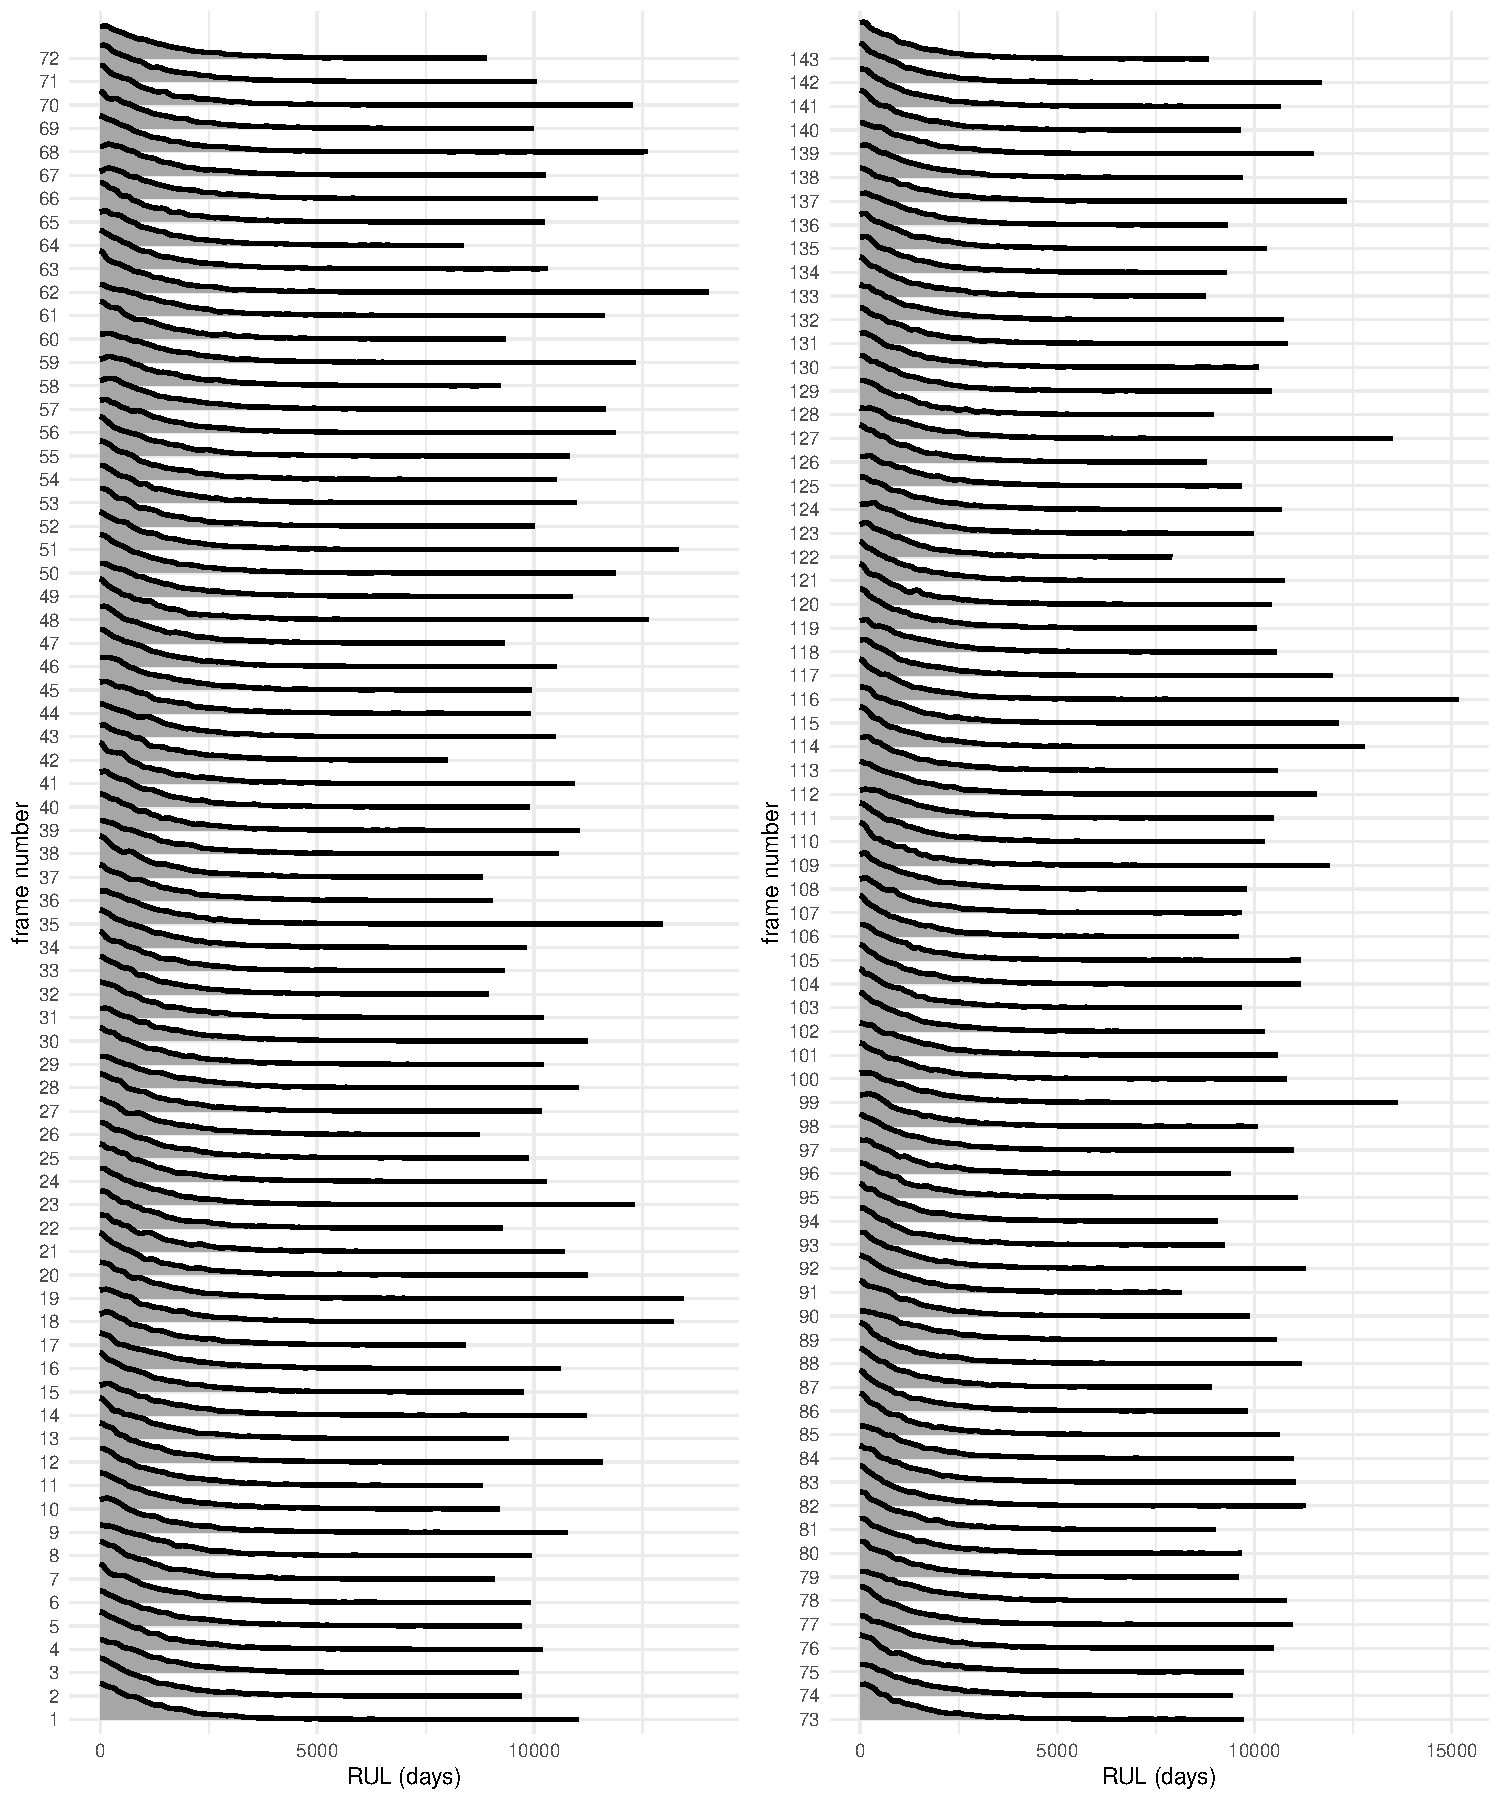
\includegraphics[width=1\textwidth]{./figures/ch-3/posterior-FTs.pdf}
  \caption{The remaining useful life distributions for the current lifetimes (the lifetimes right censored by the end of observation). The left column shows frames $1$ to $72$, and the right shows frames $73$ through $143$.}
  \label{fig:idler-FTs}
\end{figure}

\subsection{Expected number of failures} \label{subsec:idler-cumulative-failrues}

With each draw from the posterior, I obtain a set of imputed values for the lifetimes of the idler frames still in operation and, with this, a prediction of the remaining useful life. Using the draws of RUL, I can calculate the cumulative failures going forward from the end of the observation period. Using an adaptation of the notation of \citet[sec.~6]{hong2009}, the number of failures at $t$ days from the end of the observation period is $K = \sum^{n}_{i = 1}I_i$, where $I_i = 1$ if $RUL_i < t$ and $I_i = 0$ if $RUL_i > t$, and the $RUL_i$ are calculated as in \eqref{eq:idler-rul}. I express this step function as $F_K(t|\hbox{RUL}^s, \theta^s)$. Figure~\ref{fig:E-Nfailrues-draws} shows ten draws of $F_K(t|\hbox{RUL}^s, \theta^s)$.

Using the resulting distribution of $F_K(t|\hbox{RUL}, \theta)$, we can calculate the predictive distribution for the number of failures at any time $t$ in the future. Figure~\ref{fig:E-Nfailrues-densities} shows the predictive densities for the number of failures within the next one (Fig.~\ref{fig:E-Nfailrues-densities}~(a)), three (Fig.~\ref{fig:E-Nfailrues-densities}~(b)), and six (Fig.~\ref{fig:E-Nfailrues-densities}~(c)) months. From the draws that make up the distributions shown in the figure, obtaining the posterior estimates and uncertainty intervals is straightforward. Such distributions are useful for managing risk in the short term and planning, for example, managing the inventory of replacement idlers kept on site.

\begin{figure}
  \centering
  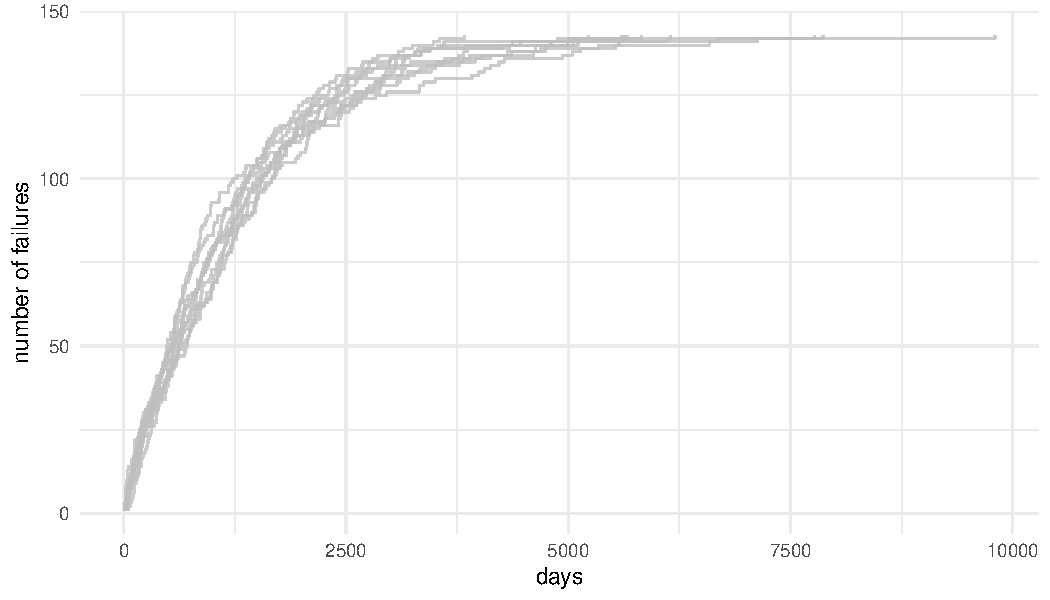
\includegraphics[width=1\textwidth]{./figures/ch-3/E-n-failures-draws.pdf}
  \caption{Ten draws of the cumulative failures proceeding the end of the observation period. The horizontal axis is the days since the end of the observation period, and the vertical axis is the cumulative number of failures.}
  \label{fig:E-Nfailrues-draws}
\end{figure}

\begin{figure}
  \centering
  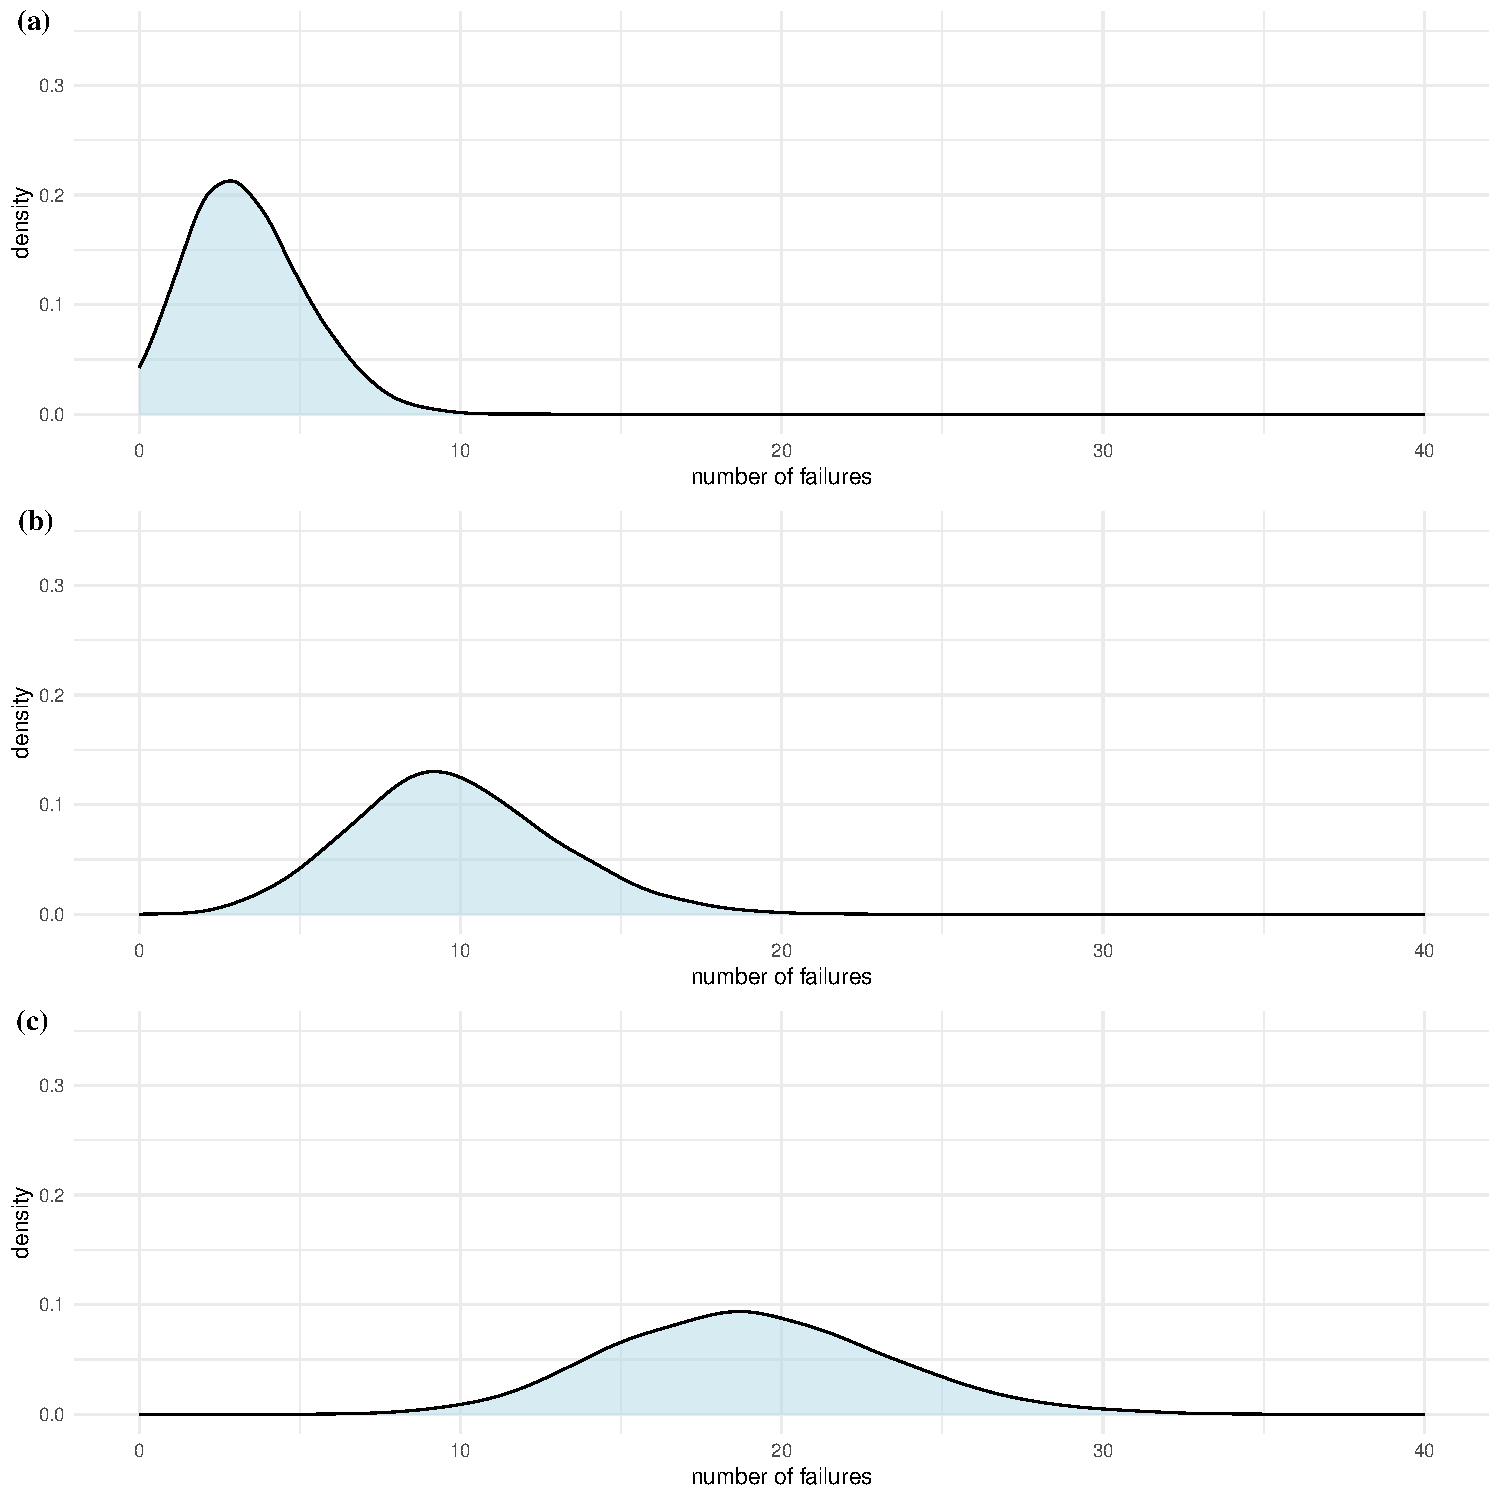
\includegraphics[width=0.7\textwidth]{./figures/ch-3/E-n-failures-densities.pdf}
  \caption{The predictive distributions for the number of failures in the one (a), three (b), and six (c) month period after the end of the observation period.}
  \label{fig:E-Nfailrues-densities}
\end{figure}

\subsection{Cost functions and preventative policy design} \label{subsec:idler-cost-function}

Construct my own cost function around the ones presented in Jardine.

Assumptions
\begin{itemize}
  \item Shuts are every six weeks. $t_p$ is the replacement interval and therefore must be a multiple of six.
  \item $N$ is the number of idler frames on the belt.
  \item $C_p$ is the cost of a preventative replacement.
  \item When an idler frame fails during operation, there is a $P = 0.1$ chance that it will damage the belt. $C_f$ is the cost of unexpectedly replacing the belt.
  \item The expected number of failures, $E(N_f)$, in a time interval $t_p$ is $N \times F_{\theta|y}(t_p)$.
  \item The probability that at least one unplanned idler failure damages the belt during the interval is $1 - (1 - P)^{N F_{\theta|y}(t_p)}$.
\end{itemize}

\begin{equation}
  \text{Cost per unit time} = \frac{C_p N + C_f (1 - (1 - P)^{N F_{\theta|y}(t_p)})}{t_p}
\end{equation}

$F_{\theta|y}(t_p)$ is the posterior CDF of the Weibull distribution (the failure time distribution). Hence, we can average over the uncertainty in the posterior draws to get the expected cost per unit time and uncertainty estimates by calculating the cost function for every posterior draw; $F_{\theta^s}(t_p)$.

If we calculate this for the set of possible shut periods we can compare the choices with uncertainty.

In this example, I have not accounted for the possibility that the belt could be damages, replaced, and then damaged again in a single interval! Jardine talks about some methods for expected number of repeat failures in a time interval in section 2.4.3

This is just a demonstration on how to use the full posterior in the decision making process.

\section{Discussion and conclusions} \label{sec:idler-frame-conclusions}

Typical results section.

\begin{itemize}
  \item Summarise main points and usefulness of chapter.
  \item In an ideal world we would analyse the failure distribution of the idlers themselves, but unfortunately the data is not available at this level. The effect of modelling the frame lifetime (which is the shorter lifetime of the three idlers it contains) is that the shape parameter is close to one---shown in the prior-data conflict. The beta value close to one makes the cost function...
  \item I've demonstrate how imputing the censored observations in a Bayesian approach provides a very natural straightforward way of obtaining estimates and uncertainty intervals for the RUL of the frames still in operation and the predicted cumulative number of failures.
  \item expected RUL and expected failures are useful for short term decision making, for example inventory of replacement idlers kept at the mine (most of these mines are fly-in-fly-out).
  \item This model could include covariates, say if manufacturer type was available---which it is for the recent idler failures---or location on the belt---impact idlers, tail or head idlers, and typical carry idlers.
  \item The method could be explored to include a mixture of failure modes to include the idlers that fail at $t < 21$, which I threw out before analysis \citep{mittman2013}. However, this would require a better understanding of the imputation method, since truncation would make it less likely that we observe the early failure mode and right censoring the longer failure mode.
\end{itemize}